\documentclass[10pt, a4paper]{article}
\usepackage{latexsym}
\usepackage{amssymb,amsmath}
\usepackage[pdftex]{graphicx}
\newcommand{\dbar}[1]{\Bar{\Bar{#1}}}

\topmargin = 0.1in \textwidth=5.7in \textheight=8.6in

\oddsidemargin = 0.1in \evensidemargin = 0.1in

% headers
\usepackage{fancyhdr}
\pagestyle{fancy}
\chead{} 
\rhead{\thepage} 
% footer
\lfoot{\small\scshape } 
\cfoot{} 
%%%% insert your name here %%%%
\rfoot{\footnotesize Michael Burton} 
\renewcommand{\headrulewidth}{.3pt} 
\renewcommand{\footrulewidth}{.3pt}
\setlength\voffset{-0.25in}
\setlength\textheight{648pt}

\begin{document}

\title{}
\author{Michael Burton}
\maketitle

\section*{Assumptions}

\begin{enumerate}
\item Fixed Engine Weight $ W_{eng-tot} \gets 6~\mathrm{lbf} \text{ } P_{shaft-maxMSL} \gets 2.189~\mathrm{kW} $.  Also assuming that engine performance is affected by altitude and RPM. This BSFC model is technically fit for a single propellor.  We are assuming that the the variance in BSFC curves in the family of propellers is small.  
\item Fixed range to station $ R \gets 200~\mathrm{nmi} $
\item Fixed payload $ W_{pay} \gets 10~\mathrm{lbf} \text{ } Vol_{pay} \gets 0.5~\mathrm{ft^{3}} $
\item Fixed altitude at cruise $ h_{cruise} \gets 5000~\mathrm{ft} $
\item Fixed altitude at station $ h_{station} \gets 1.5 \times 10^{4}~\mathrm{ft} $
\item Fixed avonics $ Vol_{avionics} \gets 0.125~\mathrm{ft^{3}} \text{ } W_{avionics} \gets 8~\mathrm{lbf} $
\item Fixed climb rate $ h_{dot} \gets 125~\mathrm{\tfrac{ft}{min}} $
\item Fixed time to get on station  $ t_{cruise} \leq 1~\mathrm{day} $
\item Constant wind speed during loiter $ V_{wind} \gets 25~\mathrm{m/s} $
\item Fuselage fineness ratio $ fr \gets 3.5 $
\end{enumerate}
\newpage

\section*{Performance Curves}

The following curves are performance curves.  They assume that the weight of the aircraft is fixed. All of the above assumptions hold.  

\begin{figure}[h!]
\begin{center}
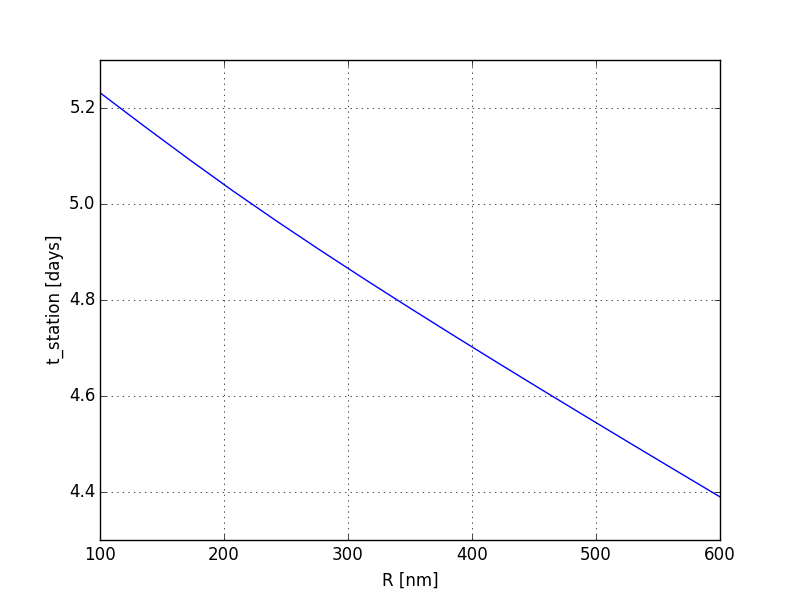
\includegraphics[scale = .5]{tvsR}
\caption{Time on station vs R. Assumes fixed weight of $MTOW = 87$ [lbf].}
\end{center}
\end{figure}

\begin{figure}[h!]
\begin{center}
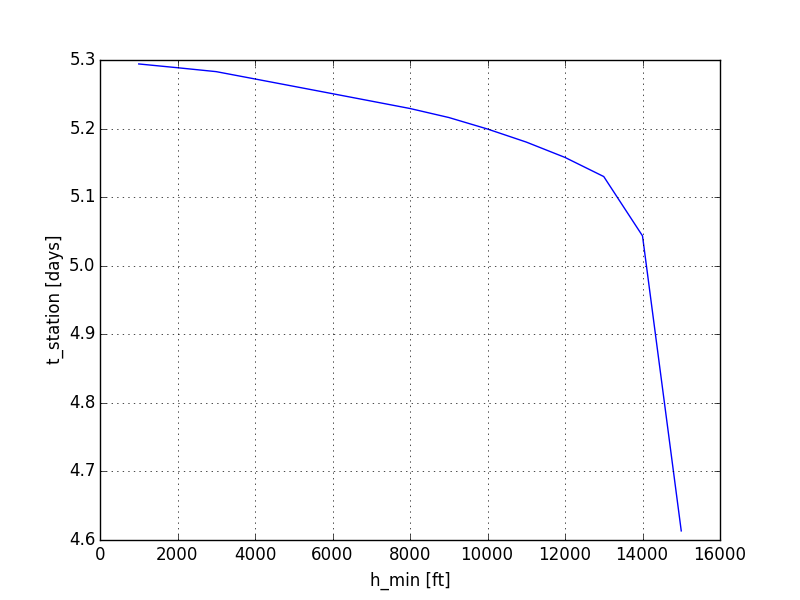
\includegraphics[scale = .5]{tvsh_min}
\caption{Time on station vs cruise altitude. Assumes fixed weight of $MTOW = 87$ [lbf].}
\end{center}
\end{figure}

\newpage

\begin{figure}[h!]
\begin{center}
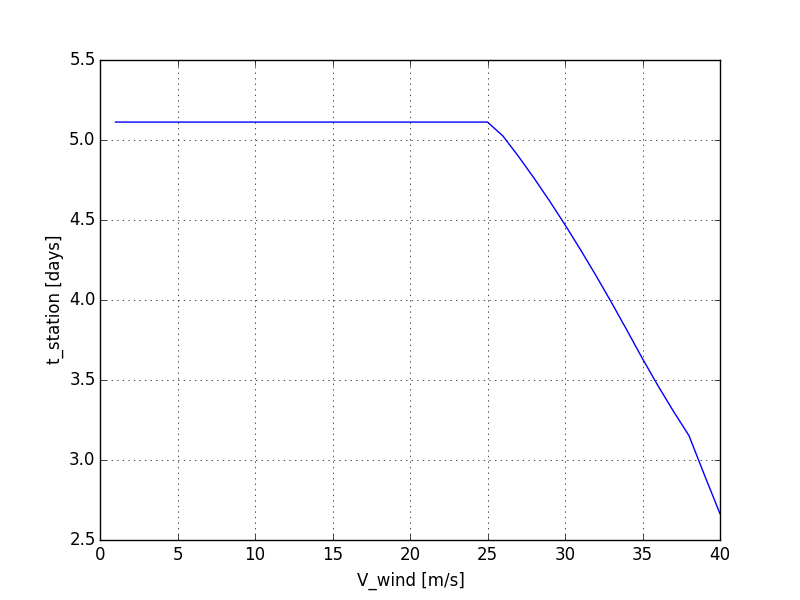
\includegraphics[scale = .5]{tvsV_wind}
\caption{Time on station vs wind velocity.  Assumes fixed weight of $MTOW = 87$ [lbf].}
\end{center}
\end{figure}

\begin{figure}[h!]
\begin{center}
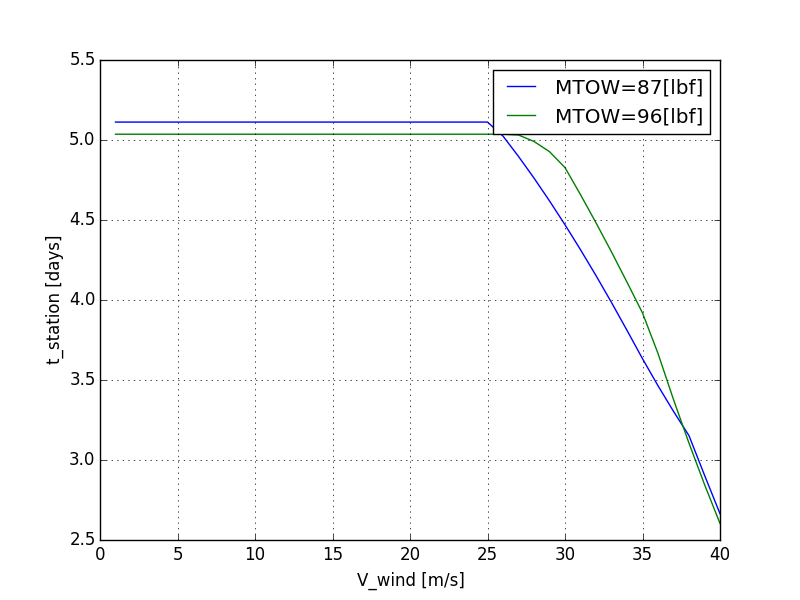
\includegraphics[scale = .5]{tvsV_wind96}
\caption{Time on station vs wind velocity. } 
\end{center}
\end{figure}

\newpage

\section*{Solution}
\begin{verbatim}

Cost
----
 83.13 [lbf] 

                 AR : 27.87                 Aspect ratio      
        A_{capcent} : 9.979e-05   [m**2]    Cap area at center      
         C_{D-fuse} : 0.003734              fueslage drag     
         C_{f-fuse} : 0.006756              Fuselage skin friction coefficient
                  F : 1633        [N]       Load on wings     
             LoverA : 5.225       [lbf/ft**2] Wing loading      
               MTOW : 83.13       [lbf]     max take off weight     
             M_cent : 1310        [N*m]     Center bending moment       
            P_{cap} : 4.74e+04    [N]       Cap load      
                  S : 15.91       [ft**2]   wing area     
           S_{fuse} : 7.994       [ft**2]   Fuselage surface area       
          Vol_{cap} : 0.0002135   [m**3]    Cap volume        
         Vol_{fuel} : 0.02653     [m**3]    Fuel Volume       
         Vol_{fuse} : 0.04423     [m**3]    fuselage volume     
           W_{cent} : 73.41       [lbf]     Center aircraft weight      
       W_{fuel-tot} : 42.13       [lbf]     total fuel weight     
           W_{fuse} : 4.284       [lbf]     fuselage weight     
           W_{wing} : 7.514       [lbf]     Total wing structural weight      
            W_{zfw} : 41          [lbf]     Zero fuel weight      
       \delta_{tip} : 4.211       [ft]      Tip deflection      
          \rho_{sl} : 1.225       [kg/m**3] density at sea level        
                  b : 21.06       [ft]      Span      
                  c : 0.7556      [ft]      Wing chord        
           h_{spar} : 0.02764     [m]       Spar height       
           l_{cent} : 2.675       [ft]      center fuselage length      
           l_{fuse} : 3.316       [ft]      fuselage length     
            m_{cap} : 0.3757      [kg]      Cap mass      
           m_{fuse} : 0.7427      [kg]      fuselage mass     
           m_{skin} : 2.956       [kg]      Skin mass     
            w_{cap} : 5.524       [in]      Spar cap width      
           w_{cent} : 0.7642      [ft]      center fuselage width       
         \vec{BSFC} : [ 0.507     0.681     0.507     0.649    ... ]  [lb/hp/hr]  brake specific fuel consumption   
          \vec{C_D} : [ 0.0304    0.0131    0.0299    0.0274   ... ]        Drag coefficient      
          \vec{C_L} : [ 1.08      0.498     1.06      0.991    ... ]        Lift coefficient      
     \vec{L_factor} : [ 0.188     0.189     0.518     0.518    ... ]        Max shaft power loss factor     
\vec{P_{shaft-max}} : [ 2.38      2.37      1.41      1.41     ... ]  [hp]      Max shaft power at altitude     
    \vec{P_{shaft}} : [ 2.38      0.66      1.41      0.448    ... ]  [hp]      Shaft power       
          \vec{RPM} : [ 8.44e+03  5.82e+03  8.44e+03  6.1e+03  ... ]  [rpm]     Engine operating RPM        
    \vec{Re_{fuse}} : [ 1.49e+06  2.18e+06  1.24e+06  1.24e+06 ... ]        fuselage Reynolds number      
           \vec{Re} : [ 3.38e+05  4.97e+05  2.83e+05  2.83e+05 ... ]        Reynolds number     
            \vec{T} : [ 9.54      2.16      4.74      2.1      ... ]  [lbf]     Thrust      
            \vec{V} : [ 20.9      30.7      25      25     ... ]  [m/s]     cruise speed      
      \vec{W_{end}} : [ 82.8      81.4      80.6      71.6     ... ]  [lbf]     segment-end weight      
     \vec{W_{fuel}} : [ 0.288     1.4     0.83      9.06     ... ]  [lbf]     segment-fuel weight     
  \vec{\eta_{prop}} : [ 0.5     0.6     0.5     0.7      ... ]        propulsive efficiency       
         \vec{\rho} : [ 1.05      1.05      0.738     0.738    ... ]  [kg/m**3]   air density       
       \vec{c_{dp}} : [ 0.0117    0.00622   0.012     0.0112   ... ]        wing profile drag coeff     
      \vec{h_{dot}} : [ 357     148      ]      [ft/min]    Climb rate        
            \vec{h} : [ 5e+03     5e+03     1.5e+04   1.5e+04  ... ]  [ft]      altitude      
            \vec{t} : [ 0.00973   0.126     0.047     1.2      ... ]  [day]     time per flight segment     
      \vec{z_{bre}} : [ 0.0034    0.0167    0.01      0.117    ... ]        breguet coefficient

Constants
---------
        BSFC_{min} : 0.32         [kg/hr/kWMinimum BSFC     
         C_{L-max} : 1.5                    Maximum lift coefficient     
           E_{cap} : 2e+07        [pound_force_per_square_inch] Youngs modulus of CF cap     
       FuelOilFrac : 0.98                   Fuel-oil fraction        
          K_{fuse} : 1.1                    Fuselage form factor     
           N_{Max} : 5                      Load factor      
  P_{shaft-maxMSL} : 2.93         [hp]      Max shaft power at MSL     
                 R : 200          [nmi]     range to station     
         RPM_{max} : 9000         [rpm]     Maximum RPM      
        R_{cruise} : 180          [nmi]     range to station during climb  
          Re_{ref} : 3e+05                  Reference Re for cdp     
          V_{wind} : 25           [m/s]     wind speed     
    Vol_{avionics} : 0.125        [ft**3]   Avionics volume      
         Vol_{pay} : 0.5          [ft**3]   Payload volume     
      W_{avionics} : 8            [lbf]     Avionics weight      
       W_{eng-tot} : 6            [lbf]     Installed engine weight      
           W_{pay} : 10           [lbf]     Payload weight     
          W_{skid} : 3            [lbf]     skid weight      
  \delta_{tip-max} : 0.2                    max tip deflection ratio     
 \eta_{prop-climb} : 0.5                    propulsive efficiency in climb 
\eta_{prop-cruise} : 0.6                    propulsive efficiency in cruise
\eta_{prop-loiter} : 0.7                    propulsive efficiency in loiter
               \mu : 1.5e-05      [N*s/m**2]Dynamic viscosity        
        \rho_{cap} : 1.76         [g/cm**3] Density of CF cap        
       \rho_{fuel} : 6.01         [lbf/liquid_gallon]     density of 100LL     
       \rho_{skin} : 0.1          [g/cm**2] Wing Skin Density        
      \sigma_{cap} : 4.75e+08     [Pa]      Cap stress     
              \tau : 0.12                   Airfoil thickness ratio      
                 e : 0.9                    Spanwise efficiency      
                fr : 3.5                    fineness ratio fuselage      
                 g : 9.81         [m/s**2]  Gravitational acceleration     
           h_{min} : 5000         [ft]      minimum cruise altitude      
       h_{station} : 1.5e+04      [ft]      minimum altitude at station    
        k-{2-fuse} : 5.938                  fuselage form factor 2     
        k_{1-fuse} : 2.858                  fuselage form factor 1     
           m_{rib} : 1.2          [kg]      rib mass       
          m_{tail} : 1            [kg]      tail mass      
           t_{cap} : 0.028        [in]      Spar cap thickness       
	t_{cruise} : 1            [day]     time to station      
       t_{station} : 6            [day]     time on station 

\end{verbatim}

\end{document}
